\documentclass{article}
\usepackage[utf8]{inputenc}
\usepackage{graphicx}
\usepackage{epstopdf}
\usepackage{caption}
\usepackage{subcaption}
\usepackage{multirow}
\usepackage{hyperref}
\usepackage{url}
\usepackage{seqsplit}
\hypersetup{pdfstartview={FitH null null null}}
\usepackage{amssymb,amsmath}
\usepackage{amsthm}
\usepackage{empheq}
\usepackage{algorithm,algpseudocode}
\usepackage[margin=1.5in]{geometry}
\usepackage{listings}
\usepackage{program}
\lstset{language=Python} 

\usepackage{listings}
\usepackage{color} %red, green, blue, yellow, cyan, magenta, black, white
\definecolor{mygreen}{RGB}{28,172,0} % color values Red, Green, Blue
\definecolor{mylilas}{RGB}{170,55,241}


\title{Ab-initio modeling using fragment matching, simulated annealing and an energy function}
\author{Caiwei Wang, Xiaokai Qian, Sean Lander, \\Haipei Fan, Puneet Gaddam, Brett Koonce\\\\University of Missouri - Columbia}

\date{March 10, 2013}

\algloopdefx{NoEndIf}[1]{\textbf{If} #1 \textbf{then}}

\begin{document}

\maketitle

\section{Abstract}
Our goal is to develop a simple prototype of fragment assembly template-free modeling system. First, we convert a collection of PDB's into residue-torsion pairs and use a sliding window to build a fragment database. Next, we randomly build a model our our target protein from matches in the database. After initialization, we replace a randomly chose fragment with a similar (BLOSUM) one, then score the new protein model (DFIRE), and finally decide if the new protein can be accepted according to simulated annealing. Finally, we repeat this process for many steps and save statistics and models at each step for evaluation. Ultimately, we create a movie of the top-scoring protein and discuss how to improve our process.

\section{Introduction}

Template free modeling is an important technique in modern bioinformatics since not all proteins have templates. First, we begin with PDB sequences converting into torsion angles using third party tools RAMA/LIPA (part of CRONKITE). Using a sliding window algorithm, we can add millions of fragments to our database. Then, for each segment, we can do a query for a match/similar protein in the database.\\\\
We use simulated annealing to score, when the current solution’s neighbor is better, accepted. If not, we select it with a probability based on the current temperature. For our project, we implemented a basic homology modeling pipeline in python, using a number of external tools like DFIRE, PyMOL and TM-score to build/present a final visualized model.


\subsection{Pipeline}

\begin{figure}[H]
\begin{center}
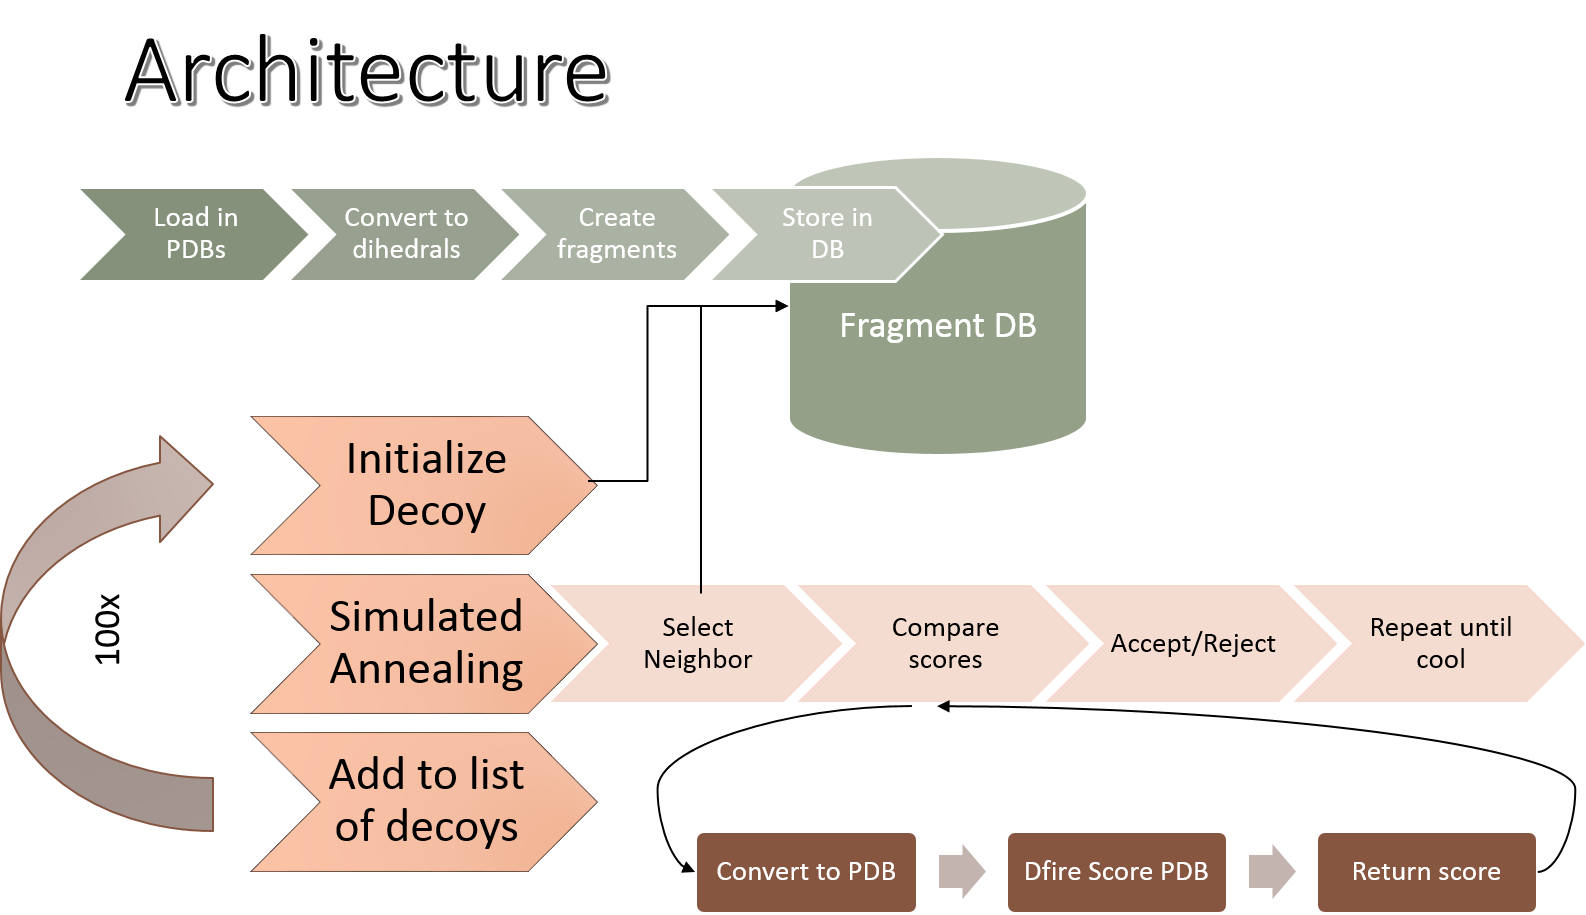
\includegraphics[width=\textwidth]{pipeline}
\caption{An overview of the TFPy pipeline}
\label{Fig:blosum}
\end{center}
\end{figure}

In order to more easily assemble our workflow we break it into a simple pipeline. Doing this allows for quick iteration on multiple fronts without the fear of breaking the model as a whole.

\begin{enumerate}

\item The first task involves building robust and well-indexed fragment databases for the three and nine length sequences. Once this is complete we are free to iterate over the simulated annealing algorithm itself.

\item Once the databases are built we create the tools necessary to initialize the candidate, choose its neighbor and score the neighbor, all of which are independent of the simulated annealing algorithm itself.

\item Initialization is less important in simulated annealing than most due to its stochastic nature, so a close approximation using fragments from the database are sufficient to build starting point.

\item Neighbor selection is more important, and fragment selection is a key component separated from the core code, as is described in our section on neighbor using Blosum62.

\item Scoring features in a similar manner, as the neighbor must be converted to a PDB file, scored with an external system, and then have its score returned and compared. In our current model D-fire energy is used to score the model.

\item Finally, multiple cooling solutions may be used, so allowing the user a choice using functional methods are preferred. We currently provide both linear and inverse-sigmoid cooling functions, with a temperature ranging from 2500 to 0 over 1000 iterations.\\

\end{steps}


Creating a system in this way leads to easy parallelization, as each decoy can be generated independent of the others. This allows for rapid decoy creation and comparison with no human component necessary beyond initial input.


\section{CASP Target goal}

We selected the following template-free targets from the CASP database to build a model for: T0693 (100 residues), T0666 (196 residues), and T0695 (537 residues).  This allows us a combination of small, medium, and large targets to test.

\section{Fragment database}

First, we selected a set of 17,000 PDB database with sequence lengths of 100-150 residues from an internal collection at MU.  For each PDB file, we split it into a list of (residue, phi angle, psi angle) chunks.  We discard the first and last residue, since they only have one valid angle.  First, we go through each PDB file sequentially for each sequence of three residues:
\begin{program}

  \FOR i:=1 \TO (length(PDB)-1)-3 \STEP 1 \DO
	a := PDB[i], b:= PDB[i+1], c:= PDB[i+2]
     	addToFragmentTrimersDatabase(a, \phi_a, \psi_a, b, \phi_b, \psi_b, c, \phi_c, \psi_c)\\\\
\END
\end{program}

Then, we repeat the process for each sequence of nine residues:
\begin{program}
  \FOR i:=1 \TO (length(PDB)-1)-9 \STEP 1 \DO
	a := PDB[i], b:= PDB[i+1], c:= PDB[i+2],  \dotso
	addToFragmentNinemersDatabase(a, \phi_a, \psi_a, b, \phi_b, \psi_b, c, \phi_c, \psi_c, \dotso)\\\\
\END
\end{program}

Finally, we create an index for each sequence in our databases, in order to speed up future lookups.  This produces a database of approximately 1.7 million sequence fragments of a reasonable size (Trimer: ~150MB, Ninemer: ~500MB) which can be searched very quickly.

\subsection{BLOSUM62 selection}

Neighbor selection is an important part of greedy and semi-greedy algorithms, as changes which are too large can disrupt the process of finding global minima and maxima. In order to generate neighbors which are close to the current sequence we use a two-fold approach: find a complete match; if a match is not found, find a match for a very similar sequence. The first approach is easy to understand, but the second requires domain knowledge of amino acids, as some acids are more similar than others.

\begin{equation*}
S_{ij}= \left( \frac{1}{\lambda} \right)\log{\left( \frac{p_{ij}}{q_i * q_j} \right)}
    \end{equation*}

The Blosum62 matrix is a pair-wise "distance" matrix of sorts which can be used to determine the similarity of two amino acids. This matrix is commonly used to determine sequence similarity for alignment purposes, but can also be used as a generative model. By finding similar amino acids to those in the current fragment sequence, we can generate multiple sequences which are very similar in terms of "distance," allowing us to expand our search criteria on limited databases.



\section{Simulated annealing algorithm}

\begin{figure}[H]
\begin{center}
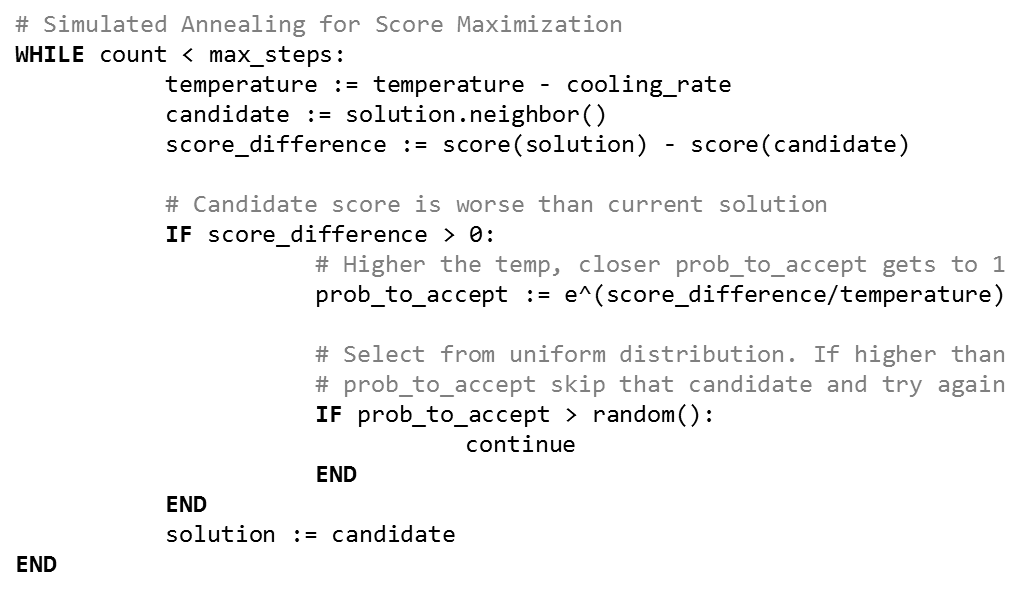
\includegraphics[width=\textwidth]{sa}
\label{Fig:blosum}
\end{center}
\end{figure}

\subsection{Simulated Annealing}

After building our fragments database, we build a initial model of our target using sequences from the database. Then, to improve our model, we use simulated annealing, a generic probabilistic metaheuristic for the global optimization problem of locating a good approximation to the global optimum of a given function in a large search space. It is often used when the search space is discrete and can prove quite efficient. Unlike hill climbing, simulated annealing can allow a poorer fragment replacement (a weaker score) early on when the function has a high temperature, which often leads to a better overall model structure. \\\\
In each cycle, we build a random neighbor of the current best solution. If the neighbor’s score is better, we promote it to  the current solution. Otherwise, we select one of the two with a probability based on the current global temperature.  Allowing a “bad” fragment replacement can allow the SA algorithm to avoid local optima.  \\\\
     This cooling schedule is an important factor in the SA algorithm. Choosing the correct parameters can efficiently and quickly help us find the optimal solution. In our project, we tested both sigmoid and linear models. We used the following candidate functions/parameters for our project:\\\\
\begin{equation*}
      T_s(k) =  -5000/(1+ exp(-k/200))+5000
    \end{equation*}
\begin{equation*}
      T_l(k) =  (-2500/1000)*k + 2500
    \end{equation*}



\subsection{d-DFIRE score}

(need a section about dDFIRE

\section{Visualization}

After we obtain a PDB file for each step of the simulated annealing process, we use PyMOL to visualize the process by displaying each model, then playing them back sequentially in the same order as they were generated.


\section{Results}

As before, our targets are: T0693 (100 residues), T0666 (196 residues), and T0695 (537 residues).  Each score contains the best result from the 9-sequence replacement pass, followed by the score from the best 3-sequence replacement pass.

\subsection{Scores}
\begin{center}
\begin{tabular}{|l|c|c|c|r|}
\multicolumn{5}{c}{T0693} \\
    \hline
      & Linear - 9 & Linear - 3 & Sigmoid - 9 & Sigmoid - 3\\ \hline
    dDFIRE & -175.6 & -177.39 & -180.98 & -194.71 \\ \hline
    TM-Score & 0.0891 & 0.0745 & 0.1162 & 0.0908 \\ \hline
    RMSD & 16.856 & 16.868 & 14.447 & 14.554 \\
    \hline
    \end{tabular}
\end{center}

\begin{center}
\begin{tabular}{|l|c|c|c|r|}
\multicolumn{5}{c}{T0666} \\
    \hline
      & Linear - 9 & Linear - 3 & Sigmoid - 9 & Sigmoid - 3\\ \hline
    dDFIRE & -75.27 & -121.34 & -82.85 & -125.35 \\ \hline
    TM-Score & 0.16113 & 0.162 & 0.1779 & 0.1565 \\ \hline
    RMSD & 23.162 & 22.569 & 25.193 & 30.457 \\
    \hline
    \end{tabular}
\end{center}

\begin{center}
\begin{tabular}{|l|c|c|c|r|}
\multicolumn{5}{c}{T0695} \\
    \hline
      & Linear - 9 & Linear - 3 & Sigmoid - 9 & Sigmoid - 3\\ \hline
    dDFIRE &  -372.27 & -375.93 & -425.11 & -431.09 \\ \hline
    TM-Score & 0.1061 & 0.1362 & 0.13 & 0.119 \\ \hline
    RMSD & 36.765 & 37.403 & 39.106 & 41.541 \\
    \hline
    \end{tabular}
\end{center}

\subsection{Future improvements}

\begin{figure}
\centering

\begin{minipage}{1.0\textwidth}
  \centering
  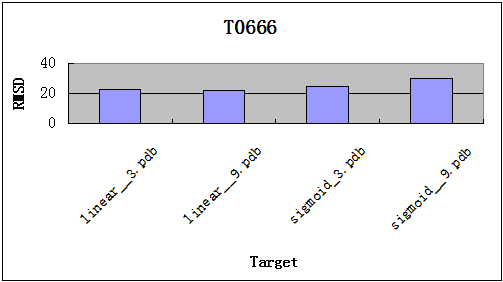
\includegraphics[width=.9\linewidth]{t0666}
  \captionof{figure}{}
  \label{fig:test1}
\end{minipage}%

\begin{minipage}{1.0\textwidth}
  \centering
  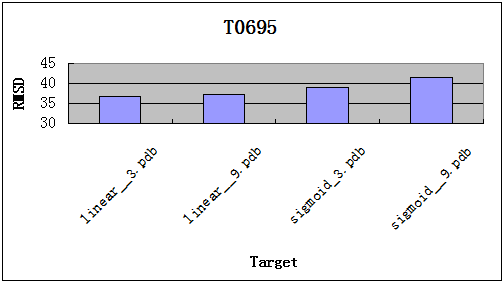
\includegraphics[width=.9\linewidth]{t0695}
  \captionof{figure}{}
  \label{fig:test2}
\end{minipage}

\begin{minipage}{1.0\textwidth}
  \centering
  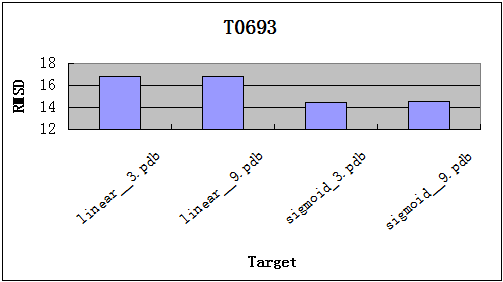
\includegraphics[width=.9\linewidth]{t0693}
  \captionof{figure}{}
  \label{fig:test2}
\end{minipage}

\end{figure}

Also we want to check whether our refinement is really good, and find out which function fits our cool schedule, we plot three histograms for each target to compare their results. From figures, we can find that our refinement can improve the quality of predictions, but only a little bit. And Linear function and sigmoid function performs well in one target, as a result, we can’t decide which one is better. We need more targets to test.


\section{Citations}

We thank the following tools and papers: \\\\




\end{document}


\end{document}
